\documentclass[9pt]{beamer}

\usepackage[version=4]{mhchem}
\usepackage[sfdefault]{FiraSans}
\usepackage{caption}
\usepackage{float}
\usepackage{pifont}

\usetheme{metropolis}
\setbeamertemplate{footline}{} %rimuove i numeri della slide
\addtobeamertemplate{frametitle}{}{\vspace{1em}} % increase
\addtobeamertemplate{frametitle}{}{\vspace{-1em}}

\setlength{\belowcaptionskip}{-10pt}
\setlength{\abovecaptionskip}{-2pt}

\beamertemplatenavigationsymbolsempty



\newcommand\blfootnote[1]{%
	\begingroup
	\renewcommand\thefootnote{}\footnote{#1}%
	\addtocounter{footnote}{-1}%
	\endgroup
}



\title{Sintesi di Composti d'Interesse Medico per il Trattamento del Morbo d'Alzheimer}
\author{
	Relatrice: Annamaria Deagostino \\
	\and
	Candidato: Lorenzo Castellino
}
\date{\center{Anno Accademico 2017-2018}}

\begin{document}

\begin{frame}
	\titlepage
\end{frame}

\begin{frame}
	\frametitle{Il Morbo d'Alzheimer in Numeri}
	Il Morbo d'Alzheimer è la prima causa di demenza a livello mondiale.

	Malattia neurodegenerativa la cui incidenza aumenta con l'avanzare dell'età.

	Stando al World Alzheimer Report del 2018:

	\begin{description}
		\item [Oggi:] 50 milioni di pazienti.

		\item [2050:] 152 milioni di pazienti.

	\end{description}

	Risulta chiaro che la ricerca di una cura sia una delle sfide del millennio. \blfootnote{World Alzheimer Report 2018 — Alzheimer’s Disease International.}
\end{frame}

\begin{frame}
	\frametitle{I $\beta$-Amiloidi e il loro Ruolo}
	\bigskip
	\begin{columns}
		\begin{column}{0.5\textwidth}
			Un $\beta$-amiloide (A$\beta$) è un particolare frammento proteico insolubile non ramificato.

			\smallskip
			Viene originato dall'azione congiunta di tre enzimi su di una proteina denominata Amyloid Precursor Protein (APP).
		\end{column}
		\begin{column}{0.5\textwidth}

			\begin{figure}
				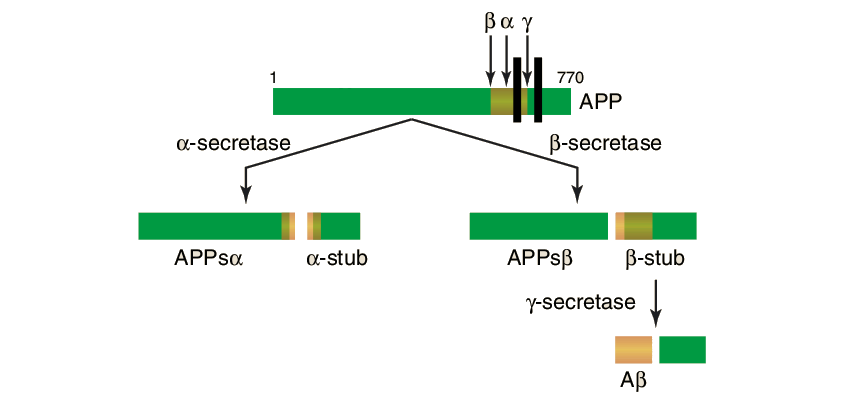
\includegraphics[width=\textwidth]{immagini/APP.png}
			\end{figure}
		\end{column}
	\end{columns}

	\medskip
	Si può presentare in due forme composte da 40 o 42 residui.

	Il frammento A$\beta$-42 se presente in grande quantità o in presenza di ioni metallici in concentrazioni anomale può dare origini a fenomeni d'aggregazione con conseguente sviluppo della patologia. \blfootnote{Goedert, M.; Spillantini, M. G. Science 2006, 314, 777–781.}

\end{frame}

\begin{frame}
	\frametitle{Come Intervenire?}
	Le metodologie d'intervento studiate nel panorama della ricerca biomedica sono molteplici.

	Nel mio lavoro mi sono soffermato su:
	\begin{itemize}
		\item Modulazione della neurotrasmissione.
		\item Mitigazione degli effetti di stress ossidativo.
		\item Limitazione dell'aggregazione dei A$\beta$.
	\end{itemize}

	Composti presi in considerazione:
	\begin{itemize}
		\item Resveratrolo %GRASSETTO
		\item Curcumina
		\item Bipiridine
	\end{itemize}


\end{frame}


\begin{frame}
	\frametitle{Resveratrolo: La Molecola}
	\begin{columns}
		\begin{column}{0.5\textwidth}
			Polifenolo presente in molte piante, principalmente nella vite.
		\end{column}
		\begin{column}{0.5\textwidth}
			\begin{figure}
				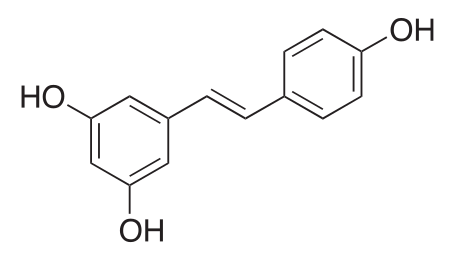
\includegraphics[width=.8\textwidth]{immagini/resveratrolo.png}
			\end{figure}
		\end{column}
	\end{columns}
	\medskip


	Potenziale candidato per il trattamento di malattie neurodegenerative viste le sue proprietà:
	\begin{itemize}
		\item Inibitore dell'enzima Acetilcolinesterasi (AChE).
		\item Riduzione delle specie ossidanti (ROI).
		\item Mitigazione della formazione di aggregati proteici.
	\end{itemize}
	\blfootnote{Jabir, N. R.; Khan, F. R.; Tabrez, S. CNS Neurosci. Ther. 2018, 24, 753–762.}
\end{frame}

\begin{frame}
	\frametitle{Resveratrolo: Sintesi I}
	\begin{figure}
		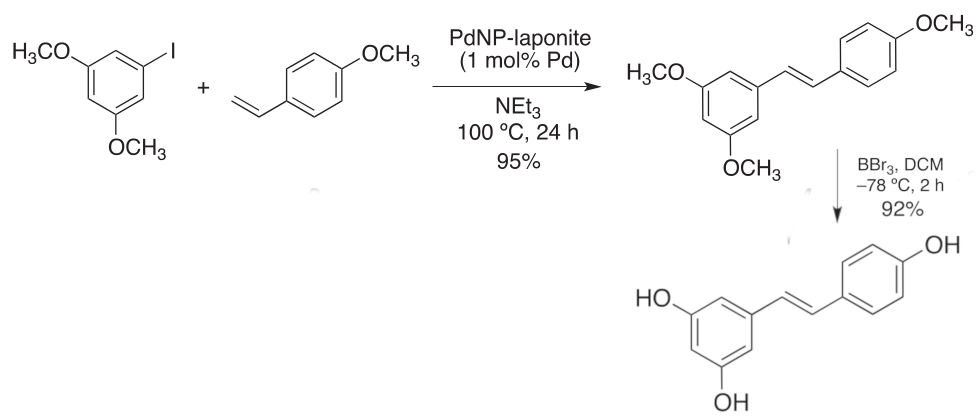
\includegraphics{immagini/totale_resveratrolo.png}
	\end{figure}
	Sintesi mediante accoppiamento Heck-Mizoroki a partire dal 1-iodo-3,5-dimetossibenzene ed il 4-metossistirene.

	Impiego di un catalizzatore al Palladio nanoparticellare disperso su di una argilla di Laponite.

	Demetilazione per mezzo di \ce{BBr3} per deproteggere i gruppi idrossilici.
	\blfootnote{Alejandro V. Martı́nez; José A. Mayoral; José I. Garcı́a Tetrahedron 2017, 73, 5581–5584.}
\end{frame}

\begin{frame}
	\frametitle{Resveratrolo: Sintesi II}
	\bigskip
	La reazione d'accoppiamento di Heck-Mizoroki è una reazione catalizzata da Palladio in grado di formare nuovi legami C-C a partire da un olefina e un alogenuro.

	\begin{figure}
		\centering
		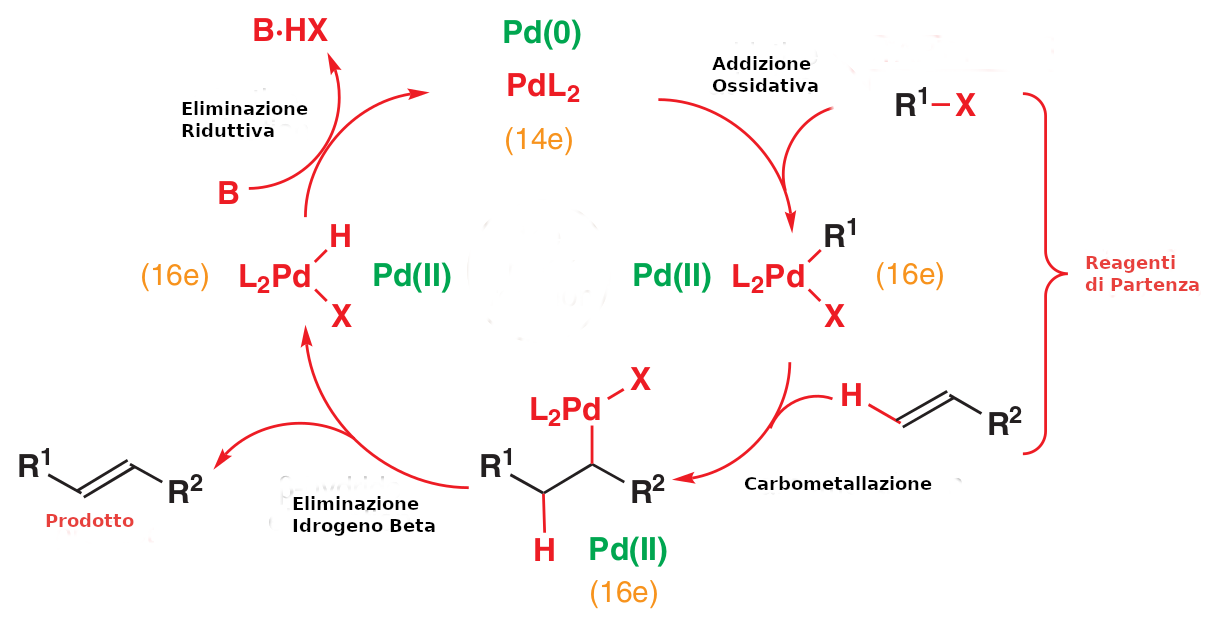
\includegraphics[width=\textwidth]{immagini/heck.png}
	\end{figure}
\end{frame}

\begin{frame}
	\frametitle{Resveratrolo: Effetti della Molecola I}
	L'azione farmacologica è stata valutata per quanto riguarda due tetrameri del Resveratrolo: Vitisina A e Heyanol A.

	Tramite un biotest HPLC sono stati valutati l'efficacia dell'inibizione dell'enzima AChE e la selettività per lo stesso.

	\begin{columns}
		\begin{column}{0.5\textwidth}
			\begin{figure}
				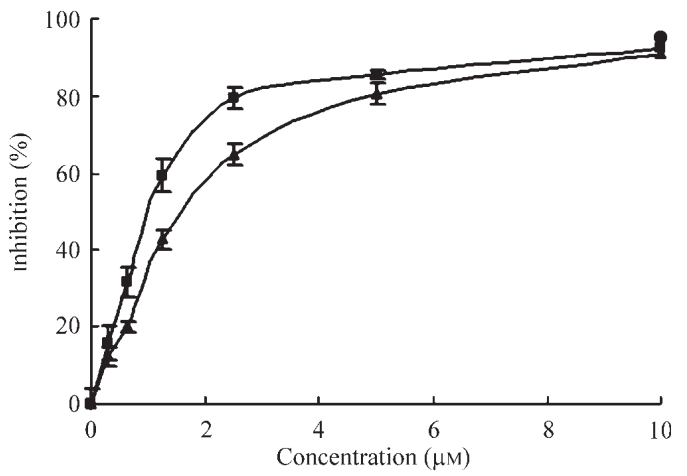
\includegraphics[width=\textwidth]{immagini/risache_resveratrolo.png}
			\end{figure}
		\end{column}
		\begin{column}{0.5\textwidth}
			\begin{figure}
				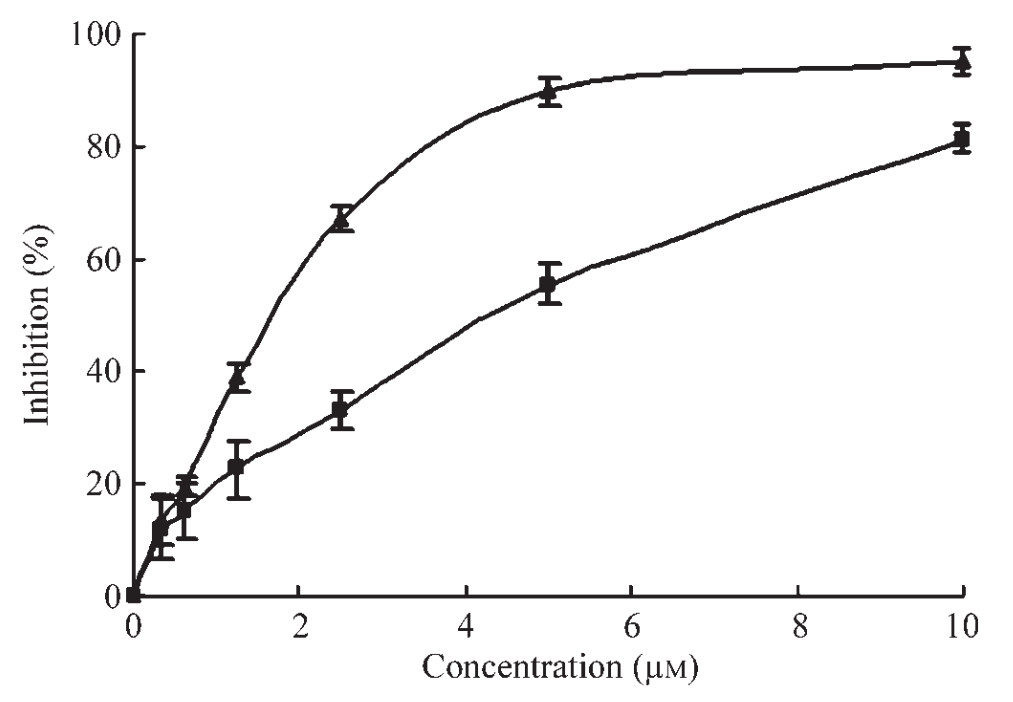
\includegraphics[width=\textwidth]{immagini/risbuche_resveratrolo.png}
			\end{figure}
		\end{column}
	\end{columns}
	Percentuale d'inibizione dell'attività degli enzimi Acetilcolinesterasi e Butirrilcolinesterasi (BuChE) per i composti Vitisina A (\ding{110}) e Heyneanol A (\ding{115})
	\blfootnote{Jang, M. H.; Piao, X. L.; Kim, J. M.; Kwon, S. W.; Park, J. H.
		Phytother. Res. 2008, 22, 544–549.}
\end{frame}

\begin{frame}
	\frametitle{Resveratrolo: Effetti della Molecola II}

	Diminuzione della mortalità cellulare e delle specie ROI in presenza di A$\beta$ in colture di cellule PC12 (feocromocitoma di ratto) opportunamente trattate.
	\begin{columns}
		\begin{column}{0.5\textwidth}
			\begin{figure}
				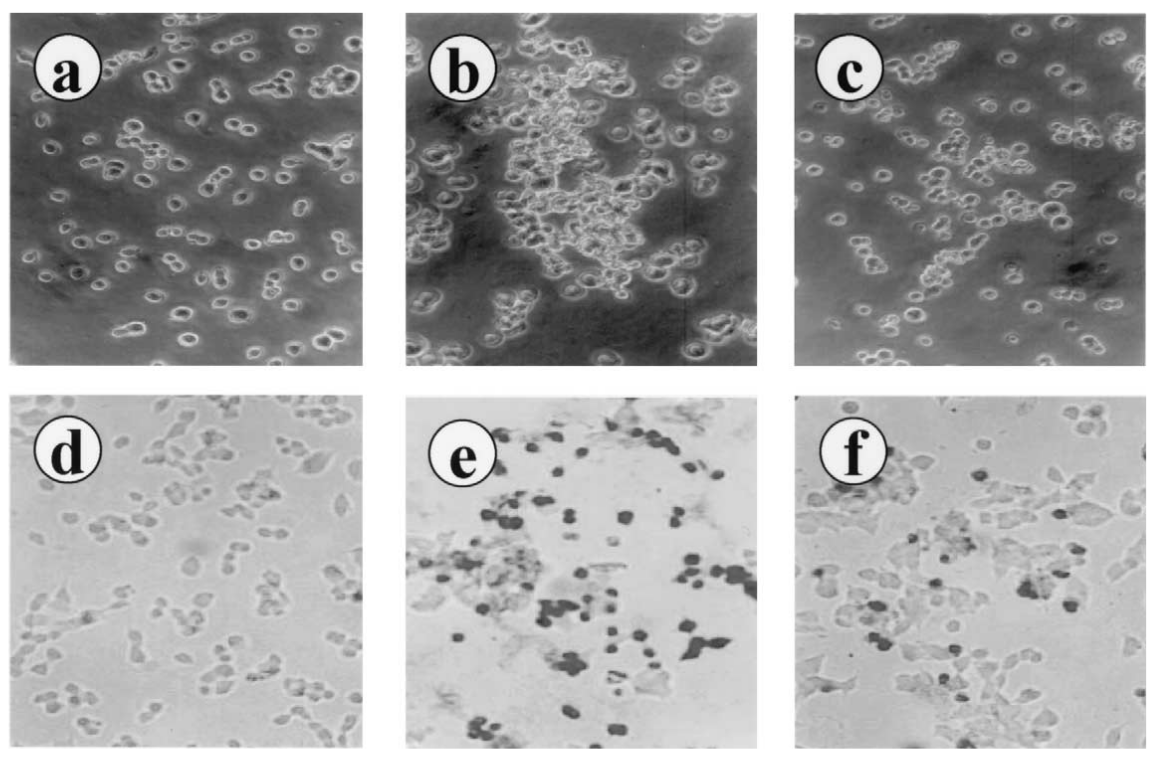
\includegraphics[width=\textwidth]{immagini/apo_resveratrolo.png}
			\end{figure}
		\end{column}
		\begin{column}{0.5\textwidth}
			\begin{figure}
				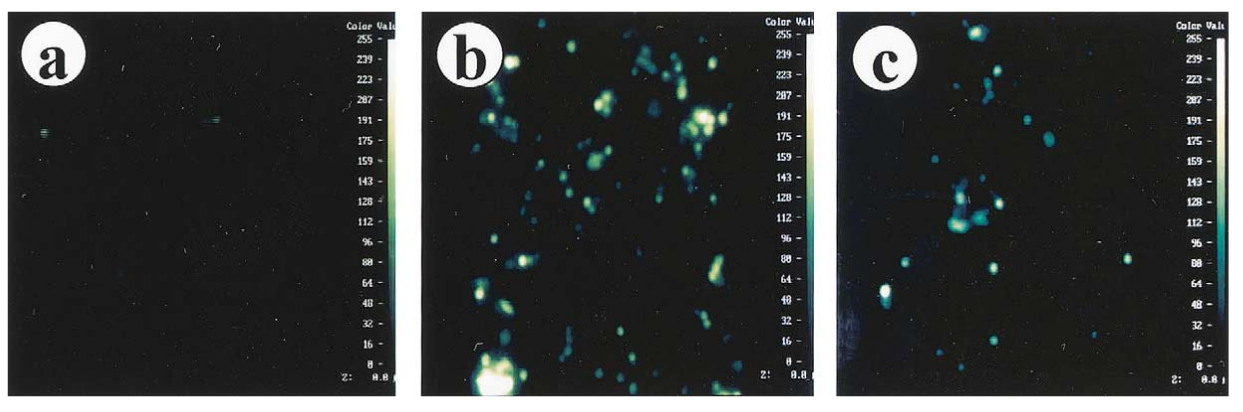
\includegraphics[width=\textwidth]{immagini/roi_resveratrolo.png}
			\end{figure}
		\end{column}
	\end{columns}
	\medskip
	\begin{columns}
		\begin{column}{0.5\textwidth}
			Cellule tal quale, in presenza di A$\beta$ e con l'aggiunta del Resveratrolo.
		\end{column}
		\begin{column}{0.5\textwidth}
			Immagine UV di cellule tal quale, in presenza di A$\beta$ e con l'aggiunta del Resveratrolo.
		\end{column}
		\blfootnote{Jang, M. H.; Piao, X. L.; Kim, J. M.; Kwon, S. W.; Park, J. H.
			Phytother. Res. 2008, 22, 544–549.}
	\end{columns}

\end{frame}


\begin{frame}
	\frametitle{Curcumina: La Molecola I}
	\begin{columns}
		\begin{column}{.4\textwidth}
			Principale componente polifenolica della Curcuma.
		\end{column}
		\begin{column}{.6\textwidth}
			\begin{figure}
				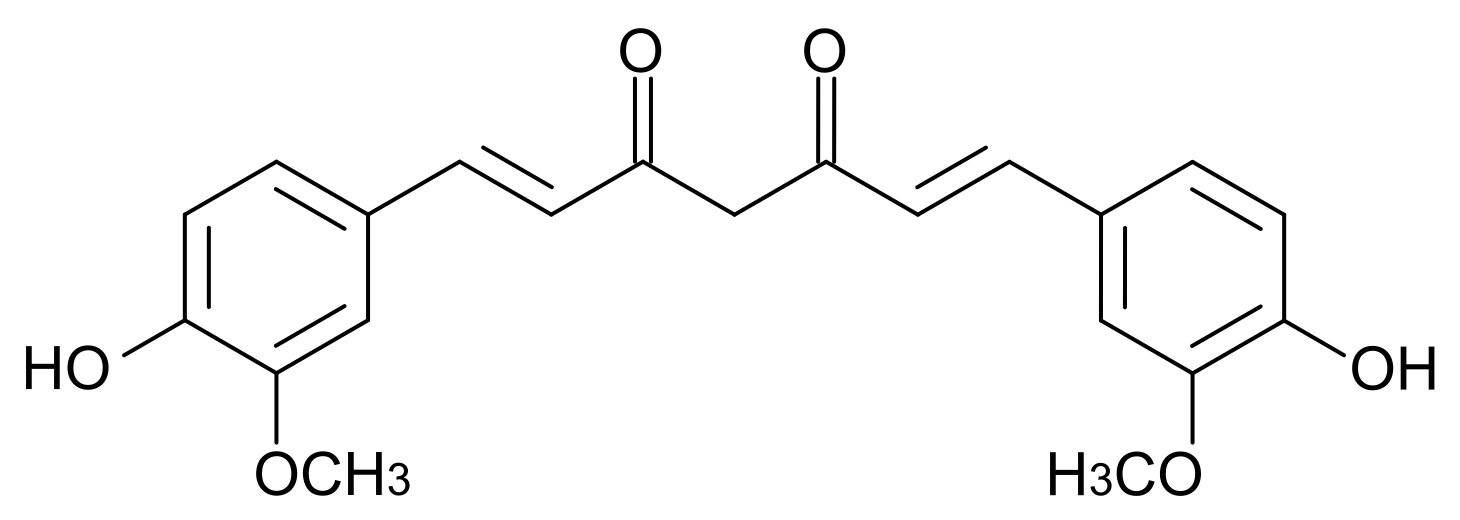
\includegraphics[width=.8\textwidth]{immagini/curcumina.png}
			\end{figure}
		\end{column}
	\end{columns}
	\bigskip

	Usata già nell'antica medicina cinese. L'azione medica è del tutto simile a quella già descritta per il Resveratrolo.

	Il principale pregio della Curcumina è la sua innata capacità di permeare la barriera emato-encefalica.

	Si può sfruttare questa proprietà accoppiando la molecola con medicinali noti per la loro azione nei confronti dell'Alzheimer come ad esempio il Donepezil.
	\blfootnote{Jun Yan; Jinhui Hu; Anqiu Liu; Lin He; Xingshu Li; Hui Wei Bioorgan. Med. Chem. 2017, 25, 2946–
		2955.}
\end{frame}

\begin{frame}
	\frametitle{Curcumina: La Molecola II}
	\begin{figure}
		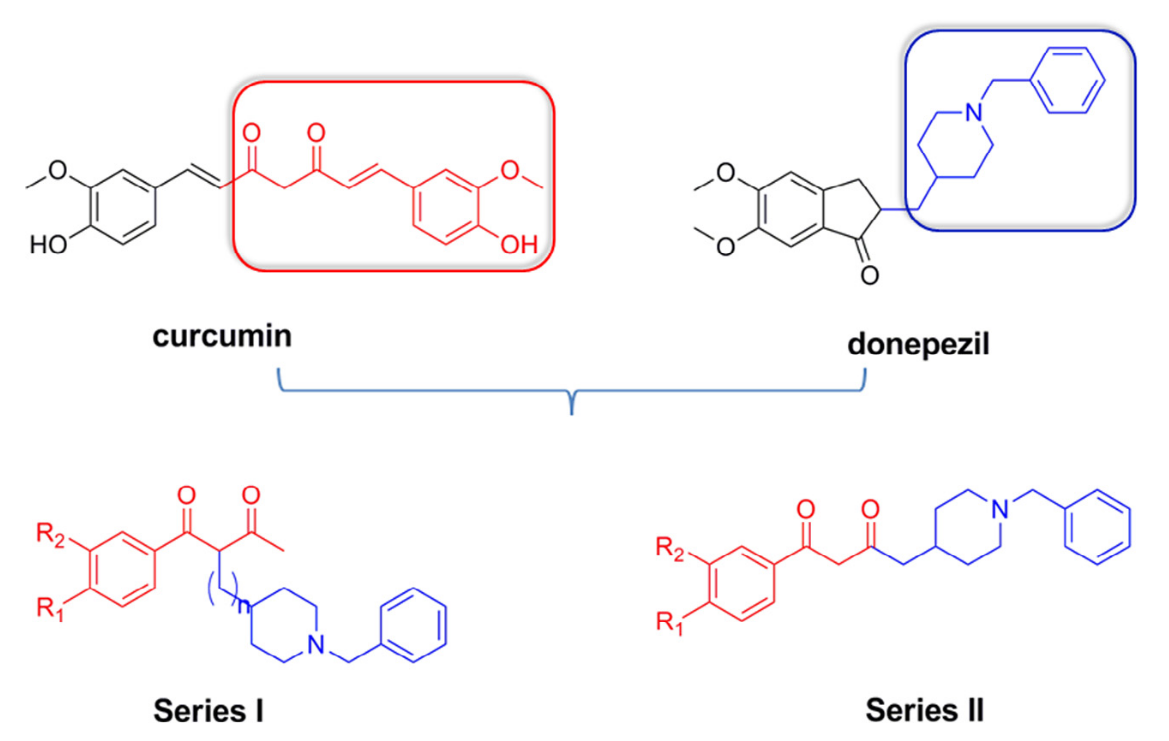
\includegraphics[scale=0.9]{immagini/generale_curcdone.png}
	\end{figure}
	\blfootnote{Jun Yan; Jinhui Hu; Anqiu Liu; Lin He; Xingshu Li; Hui Wei Bioorgan. Med. Chem. 2017, 25, 2946–
		2955.}
\end{frame}

\begin{frame}
	\frametitle{Curcumina: Sintesi I}
	A partire da reagenti commerciali sono sintetizzati i farmacofori corrispondenti per il Donepezil:
	\begin{figure}
		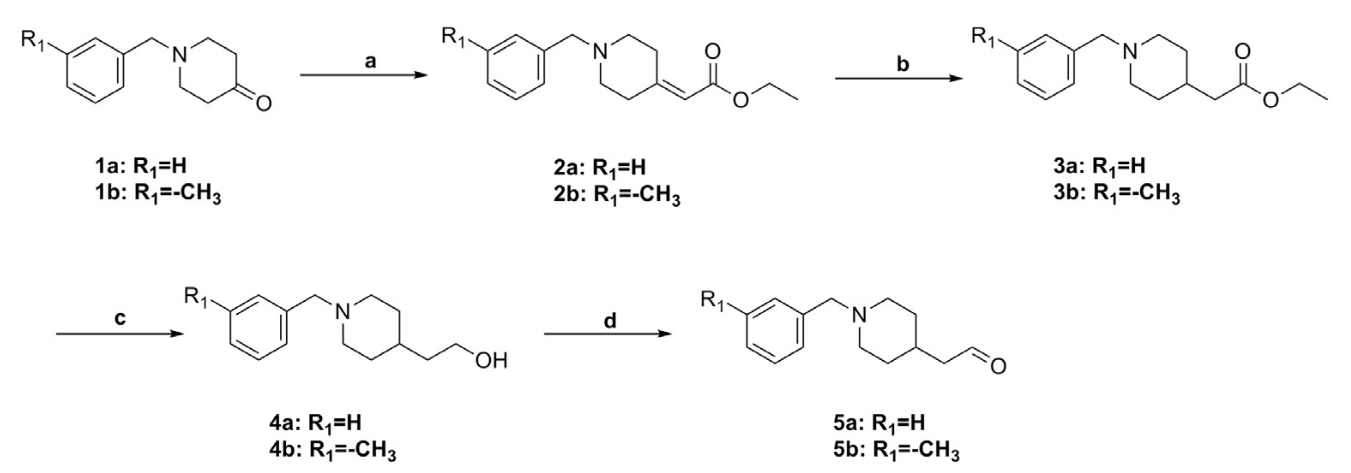
\includegraphics[width=.7\textwidth]{immagini/farmadone_curcdone.png}
		{\caption*{\tiny{(a) \ce{(EtO)2POCH2CO2Et}, \ce{K2CO3} , THF;   (b) Pd/C, \ce{H2} , \ce{MeOH};   (c) \ce{LiAlH4} , THF; (d) \ce{(COCl)2}, DMSO, \ce{N(CH2CH3)3}.}}}
	\end{figure}
	E per la Curcumina:
	\begin{figure}
		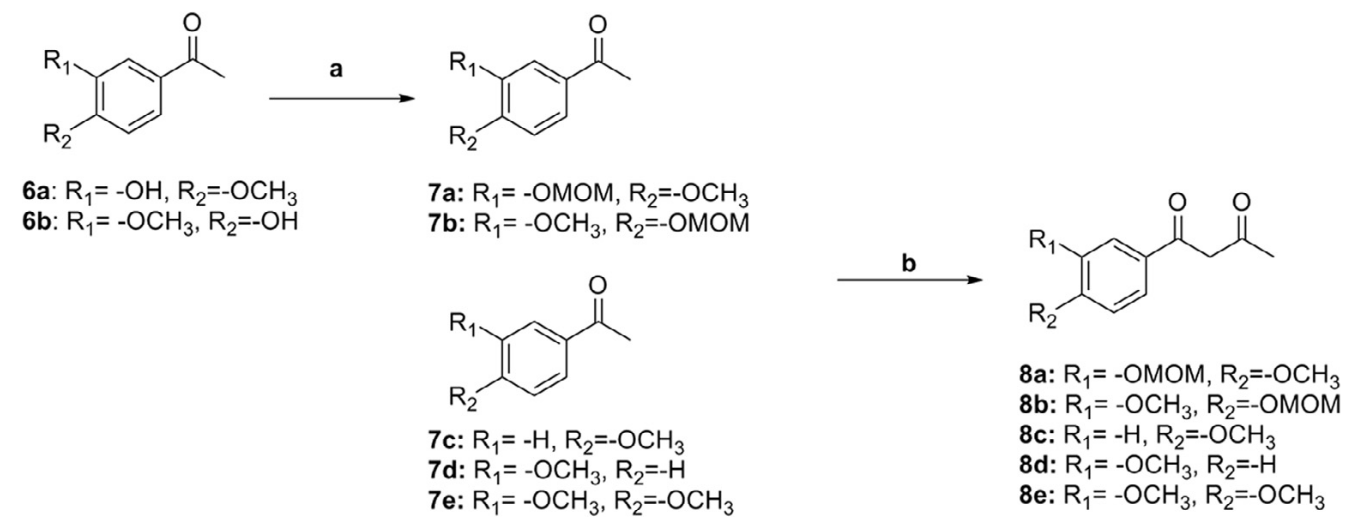
\includegraphics[width=.7\textwidth]{immagini/farmacurc_curcdone.png}
		{\caption*{\tiny{(a) \ce{MOMCl}, DIPEA, DCM; (b) \ce{NaNH2} , EtOAc, 60 $^\circ$C.}}}
	\end{figure}
\end{frame}

\begin{frame}
	\frametitle{Curcumina: Sintesi II}
	I due farmacofori ottenuti vengono accoppiati per formare i composti desiderati della prima serie per mezzo di una condensazione aldolica:
	\begin{figure}
		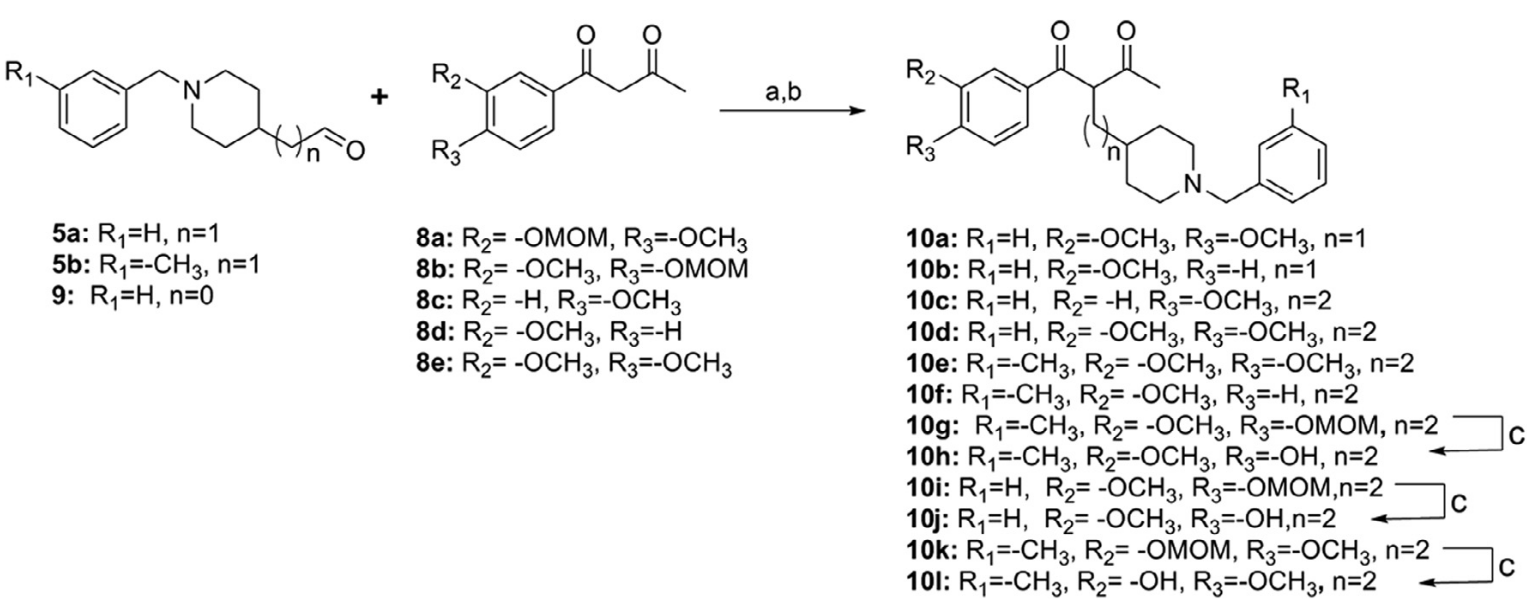
\includegraphics[width=.7\textwidth]{immagini/condserie1_curcdone.png}
		{\caption*{\tiny{(a) L-prolina, \ce{MgSO4} , EtOH, reflusso; (b) 10\% Pd/C, MeOH; (c) HCl, EtOH.}}}
	\end{figure}
	E per la seconda serie grazie ad una condensazione di Claisen:
	\begin{figure}
		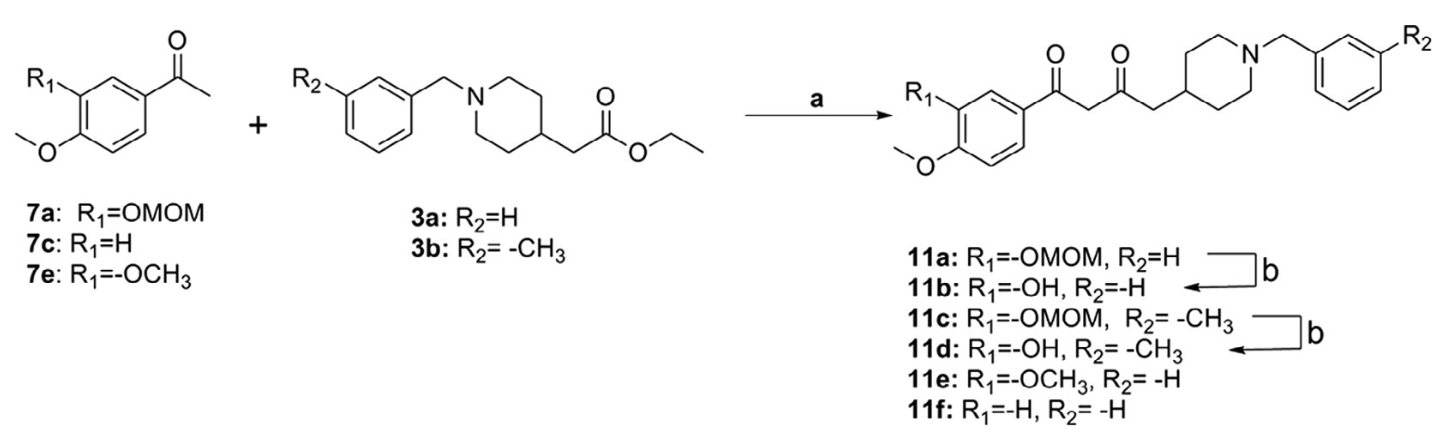
\includegraphics[width=.7\textwidth]{immagini/condserie2_curcdone.png}
		{\caption*{\tiny{(a) \ce{NaNH2} , THF, 60 $^\circ$C; (b) HCl, EtOH.}}}
	\end{figure}
	\blfootnote{Jun Yan; Jinhui Hu; Anqiu Liu; Lin He; Xingshu Li; Hui Wei Bioorgan. Med. Chem. 2017, 25, 2946–
		2955.}
\end{frame}

\begin{frame}
	\frametitle{Curcumina: Effetti delle Molecole I}

	\begin{figure}
		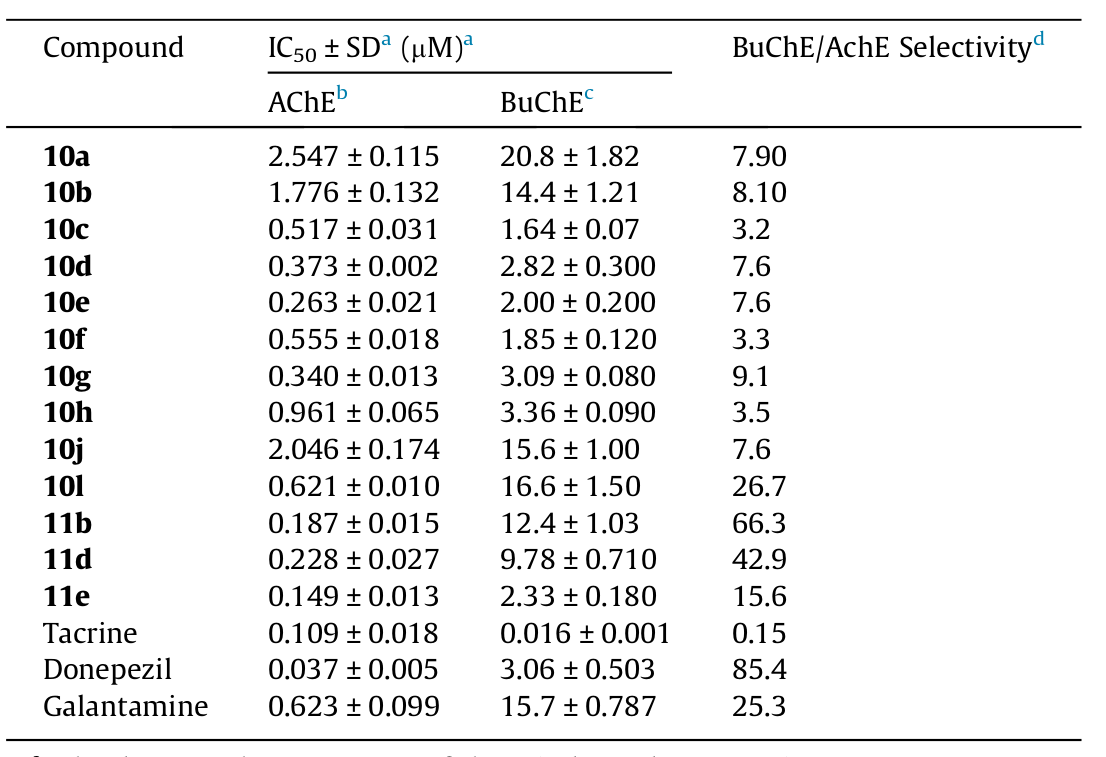
\includegraphics[scale=0.6]{immagini/tabellacomposti_curcdone.png}
		{\caption*{\footnotesize{Valutazione dell’azione nei confronti dell’AChE e selettività rispetto ad esso.}}}
	\end{figure}

	\begin{figure}
		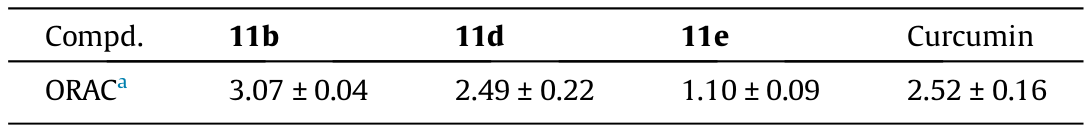
\includegraphics[scale=0.6]{immagini/roi_curcdone.png}
		{\caption*{\footnotesize{Proprietà antiossidante; valori espressi come equivalenti di Trolox.}}}
	\end{figure}

	\begin{figure}
		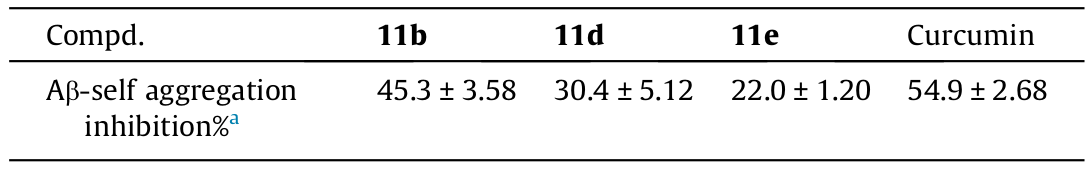
\includegraphics[scale=0.6]{immagini/selfab_curcdone.png}
		{\caption*{\footnotesize{Mitigazione dell'aggregazione amiloidica.}}}
	\end{figure}

	\small{ La permeazione della membrana emato-encefalica è risultata pressoché invariata rispetto alla Curcumina.} \medskip
	\blfootnote{Jun Yan; Jinhui Hu; Anqiu Liu; Lin He; Xingshu Li; Hui Wei Bioorgan. Med. Chem. 2017, 25, 2946–
		2955.}
\end{frame}


\begin{frame}
	\frametitle{Bipiridine: La Molecola I}
	\begin{columns}
		\begin{column}{.6\textwidth}
			Classe di composti particolarmente interessanti per il trattamento dell'Alzheimer per quanto riguarda la chelazione di metalli:
			\begin{itemize}
				\item Buona azione chelante.
				\item Costanti d'equilibrio alte per la forma complessata
				\item Buona solubilità in ambiente acquoso.
				\item Buona permeazione della barriera emato-encefalica.
			\end{itemize}
		\end{column}
		\begin{column}{.4\textwidth}
			\begin{figure}
				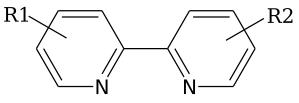
\includegraphics[width=\textwidth]{immagini/bpy.png}
			\end{figure}
		\end{column}
	\end{columns}
	\bigskip
	Introducendo funzionalità sullo scheletro molecolare l'intenzione è quella di ottenere molecole in grado di mitigare l'aggregazione in placche dei A$\beta$:
	\begin{itemize}
		\item Gruppo metilico, favorisce la chelazione.
		\item Gruppo dimetilamminico, interagisce con i A$\beta$ e favorisce la complessazione.
	\end{itemize}
	\blfootnote{Ji, Y.; Lee, H. J.; Kim, M.; Nam, G.; Lee, S. J. C.; Cho, J.; Park, C.-M.; Lim, M. H. Inorg. Chem. 2017,
		56, 6695–6705.}
\end{frame}

\begin{frame}
	\frametitle{Bipiridine: Sintesi I}
	Il processo di sintesi delle bipiridine può essere effettuato con una reazione di Stille.

	\begin{figure}
		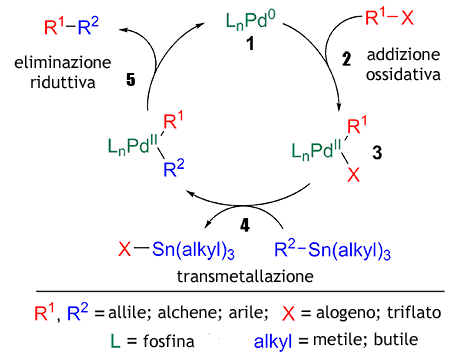
\includegraphics[scale=0.7]{immagini/stille.png}
	\end{figure}

\end{frame}

\begin{frame}
	\frametitle{Bipiridine: Sintesi II}
	\begin{figure}
		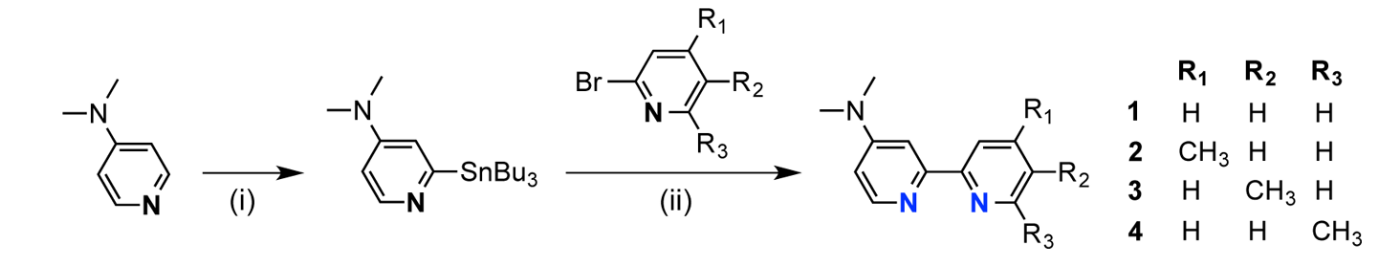
\includegraphics[width=\textwidth]{immagini/rea_g.png}
		{\caption*{\footnotesize{(i) n-BuLi, 2-Dimetilaminoetanolo, Esano, 0 $^\circ$C; \ce{Bu3SnCl}, -78 $^\circ$C; (ii) \ce{PdCl2(PPh3)2}, \ce{LiCl}, \ce{PPh3}, Toluene, 110 $^\circ$C}}}
	\end{figure}
	\begin{itemize}
		\item Si forma lo stannano a partire dalla 4-dimetilamminopiridina.
		\item Si effettua l'accoppiamento dello stannano ottenuto con la piridina bromurata tramite la reazione di Stille.
	\end{itemize}

	\blfootnote{Ji, Y.; Lee, H. J.; Kim, M.; Nam, G.; Lee, S. J. C.; Cho, J.; Park, C.-M.; Lim, M. H. Inorg. Chem. 2017,
		56, 6695–6705.}
\end{frame}

\begin{frame}
	\frametitle{Bipiridine: Effetti della Molecola}
	L'azione di composti sintetizzati è stata valutata con esperimenti in vitro

	\begin{figure}
		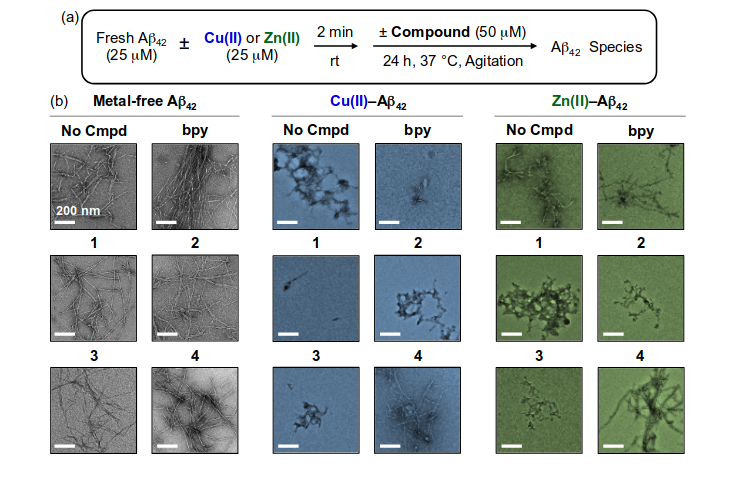
\includegraphics[scale=1.5]{immagini/ris_bpy2.png}
	\end{figure}
	\blfootnote{Ji, Y.; Lee, H. J.; Kim, M.; Nam, G.; Lee, S. J. C.; Cho, J.; Park, C.-M.; Lim, M. H. Inorg. Chem. 2017,
		56, 6695–6705.}
\end{frame}

\begin{frame}
	\frametitle{Concludendo...}
	Ad oggi una cura al Morbo d'Alzheimer non è ancora stata individuata.

	La chimica organica può fornire a medici e biochimici gli strumenti per affrontare il problema:
	\begin{itemize}

		\item Attraverso la sintesi di composti ispirati a prodotti 	presenti in natura come visto nelle sezioni relative a Resveratrolo e Curcumina.
		\item Sintetizzando molecole ad hoc sulla base delle funzionalità richieste come nel caso delle bipiridine.

	\end{itemize}
\end{frame}

\end{document}
